% Figure from MATH 591 notes, section 67 (the flow domain of X = y x^2 d/dx, sliced at y = 1). Added, not from lecture.
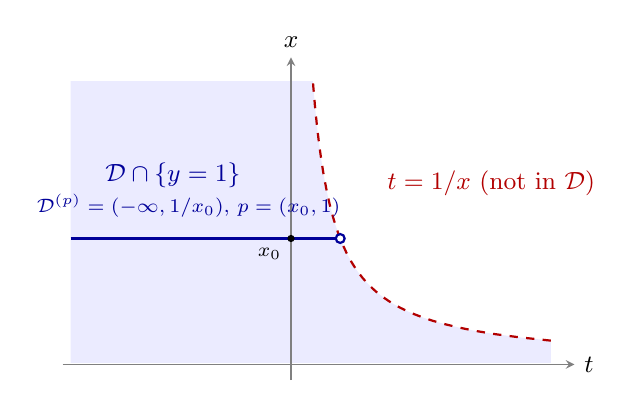
\begin{tikzpicture}[>=stealth, font=\small]
  \fill[blue!8] (-2.8,0.02) -- (3.3,0.02) -- (3.300,0.303) -- (2.901,0.345) -- (2.587,0.386) -- (2.335,0.428) -- (2.128,0.470) -- (1.954,0.512) -- (1.807,0.553) -- (1.680,0.595) -- (1.570,0.637) -- (1.474,0.679) -- (1.388,0.720) -- (1.312,0.762) -- (1.244,0.804) -- (1.183,0.846) -- (1.127,0.887) -- (1.076,0.929) -- (1.030,0.971) -- (0.988,1.013) -- (0.949,1.054) -- (0.912,1.096) -- (0.879,1.138) -- (0.848,1.179) -- (0.819,1.221) -- (0.792,1.263) -- (0.766,1.305) -- (0.743,1.346) -- (0.720,1.388) -- (0.699,1.430) -- (0.680,1.472) -- (0.661,1.513) -- (0.643,1.555) -- (0.626,1.597) -- (0.610,1.639) -- (0.595,1.680) -- (0.581,1.722) -- (0.567,1.764) -- (0.554,1.805) -- (0.541,1.847) -- (0.529,1.889) -- (0.518,1.931) -- (0.507,1.972) -- (0.496,2.014) -- (0.486,2.056) -- (0.477,2.098) -- (0.467,2.139) -- (0.458,2.181) -- (0.450,2.223) -- (0.442,2.265) -- (0.434,2.306) -- (0.426,2.348) -- (0.418,2.390) -- (0.411,2.431) -- (0.404,2.473) -- (0.398,2.515) -- (0.391,2.557) -- (0.385,2.598) -- (0.379,2.640) -- (0.373,2.682) -- (0.367,2.724) -- (0.362,2.765) -- (0.356,2.807) -- (0.351,2.849) -- (0.346,2.891) -- (0.341,2.932) -- (0.336,2.974) -- (0.332,3.016) -- (0.327,3.057) -- (0.323,3.099) -- (0.318,3.141) -- (0.314,3.183) -- (0.310,3.224) -- (0.306,3.266) -- (0.302,3.308) -- (0.299,3.350) -- (0.295,3.391) -- (0.291,3.433) -- (0.288,3.475) -- (0.284,3.517) -- (0.281,3.558) -- (0.278,3.600) -- (-2.8,3.6) -- cycle;
  \draw[->, gray] (-2.9,0) -- (3.6,0) node[right, text=black] {$t$}; \draw[->, gray] (0,-0.2) -- (0,3.9) node[above, text=black] {$x$};
  \draw[thick, red!70!black, dashed] (3.300,0.303) -- (2.901,0.345) -- (2.587,0.386) -- (2.335,0.428) -- (2.128,0.470) -- (1.954,0.512) -- (1.807,0.553) -- (1.680,0.595) -- (1.570,0.637) -- (1.474,0.679) -- (1.388,0.720) -- (1.312,0.762) -- (1.244,0.804) -- (1.183,0.846) -- (1.127,0.887) -- (1.076,0.929) -- (1.030,0.971) -- (0.988,1.013) -- (0.949,1.054) -- (0.912,1.096) -- (0.879,1.138) -- (0.848,1.179) -- (0.819,1.221) -- (0.792,1.263) -- (0.766,1.305) -- (0.743,1.346) -- (0.720,1.388) -- (0.699,1.430) -- (0.680,1.472) -- (0.661,1.513) -- (0.643,1.555) -- (0.626,1.597) -- (0.610,1.639) -- (0.595,1.680) -- (0.581,1.722) -- (0.567,1.764) -- (0.554,1.805) -- (0.541,1.847) -- (0.529,1.889) -- (0.518,1.931) -- (0.507,1.972) -- (0.496,2.014) -- (0.486,2.056) -- (0.477,2.098) -- (0.467,2.139) -- (0.458,2.181) -- (0.450,2.223) -- (0.442,2.265) -- (0.434,2.306) -- (0.426,2.348) -- (0.418,2.390) -- (0.411,2.431) -- (0.404,2.473) -- (0.398,2.515) -- (0.391,2.557) -- (0.385,2.598) -- (0.379,2.640) -- (0.373,2.682) -- (0.367,2.724) -- (0.362,2.765) -- (0.356,2.807) -- (0.351,2.849) -- (0.346,2.891) -- (0.341,2.932) -- (0.336,2.974) -- (0.332,3.016) -- (0.327,3.057) -- (0.323,3.099) -- (0.318,3.141) -- (0.314,3.183) -- (0.310,3.224) -- (0.306,3.266) -- (0.302,3.308) -- (0.299,3.350) -- (0.295,3.391) -- (0.291,3.433) -- (0.288,3.475) -- (0.284,3.517) -- (0.281,3.558) -- (0.278,3.600);
  \node[red!70!black, anchor=west] at (1.1,2.3) {$t = 1/x$ (not in $\mathcal{D}$)};
  \node[blue!60!black] at (-1.5,2.4) {$\mathcal{D} \cap \{y = 1\}$};
  \draw[thick, blue!60!black] (-2.8,1.60) -- (0.625,1.60); \draw[thick, blue!60!black, fill=white] (0.625,1.60) circle (1.6pt);
  \node[blue!60!black, anchor=south, font=\scriptsize] at (-1.3,1.74) {$\mathcal{D}^{(p)} = (-\infty, 1/x_0)$, $p = (x_0, 1)$};
  \fill (0,1.60) circle (1.3pt) node[below left, font=\scriptsize] {$x_0$};
\end{tikzpicture}
